\appendix
\chapter{Anhang}\label{ch_anhang}
\begin{figure}[h!]
    \centering
    \setlength{\fboxsep}{1pt}
    \setlength{\fboxrule}{1pt}
    \fbox{\includegraphics[width=0.92\textwidth]{C:/Users/gesc_ma/VSCode MPC Projekt/dynaovrcontroller/dynaovrcontroller/aimpoint_control_scenarios/plots/00_no_control/shading_120sec_75_30mps.png}}
    \caption[Simulationsverlauf für das Cloud Standby Referenzszenario bei Verschattung von $\SI{25}{\percent}$ und $\SI{30}{\metre\per\second}$ Wolkengeschwindigkeit]{Simulationsverlauf für das Cloud Standby Referenzszenario bei Verschattung von $\SI{25}{\percent}$ und $\SI{30}{\metre\per\second}$ Wolkengeschwindigkeit}
    \label{fig_nocontrol7530}
\end{figure}

\begin{figure}[h!]
    \centering
    \setlength{\fboxsep}{1pt}
    \setlength{\fboxrule}{1pt}
    \fbox{\includegraphics[width=0.92\textwidth]{C:/Users/gesc_ma/VSCode MPC Projekt/dynaovrcontroller/dynaovrcontroller/aimpoint_control_scenarios/plots/01_mpc_all_information/shading_120sec_75_30mps.png}}
    \caption[Simulationsverlauf für den Betrieb mit abweichungsfreier Einstrahlungsvorhersage bei Verschattung von $\SI{25}{\percent}$ und $\SI{30}{\metre\per\second}$ Wolkengeschwindigkeit]{Simulationsverlauf für den Betrieb mit abweichungsfreier Einstrahlungsvorhersage bei Verschattung von $\SI{25}{\percent}$ und $\SI{30}{\metre\per\second}$ Wolkengeschwindigkeit}
    \label{fig_allwissend7530}
\end{figure}

\begin{figure}[h!]
    \centering
    \setlength{\fboxsep}{1pt}
    \setlength{\fboxrule}{1pt}
    \fbox{\includegraphics[width=0.99\textwidth]{C:/Users/gesc_ma/VSCode MPC Projekt/dynaovrcontroller/dynaovrcontroller/aimpoint_control_scenarios/plots/00_no_control/shading_120sec_00_30mps.png}}
    \caption[Simulationsverlauf für das Cloud Standby Referenzszenario bei Verschattung von $\SI{100}{\percent}$ und $\SI{30}{\metre\per\second}$ Wolkengeschwindigkeit]{Simulationsverlauf für das Cloud Standby Referenzszenario bei Verschattung von $\SI{100}{\percent}$ und $\SI{30}{\metre\per\second}$ Wolkengeschwindigkeit}
    \label{fig_cloudstandby0030}
\end{figure}

\begin{figure}[h!]
    \centering
    \setlength{\fboxsep}{1pt}
    \setlength{\fboxrule}{1pt}
    \fbox{\includegraphics[width=0.99\textwidth]{C:/Users/gesc_ma/VSCode MPC Projekt/dynaovrcontroller/dynaovrcontroller/aimpoint_control_scenarios/plots/01_mpc_all_information/shading_120sec_00_30mps.png}}
    \caption[Simulationsverlauf für den Betrieb mit abweichungsfreier Einstrahlungsvorhersage bei Verschattung von $\SI{100}{\percent}$ und $\SI{30}{\metre\per\second}$ Wolkengeschwindigkeit]{Simulationsverlauf für den Betrieb mit abweichungsfreier Einstrahlungsvorhersage bei Verschattung von $\SI{100}{\percent}$ und $\SI{30}{\metre\per\second}$ Wolkengeschwindigkeit}
    \label{fig_allwissend0030}
\end{figure}

\begin{figure}[h!]
    \centering
    \setlength{\fboxsep}{1pt}
    \setlength{\fboxrule}{1pt}
    \fbox{\includegraphics[width=0.99\textwidth]{C:/Users/gesc_ma/VSCode MPC Projekt/dynaovrcontroller/dynaovrcontroller/aimpoint_control_scenarios/plots/02_mpc_thinking_clearsky/shading_120sec_75_20mps.png}}
    \caption[Simulationsverlauf für den Betrieb ohne Einstrahlungsvorhersage bei Lichtdurchlässigkeit der Wolke von $\SI{75}{\percent}$ und $\SI{20}{\metre\per\second}$ Wolkengeschwindigkeit]{Simulationsverlauf für den Betrieb ohne Einstrahlungsvorhersage bei Lichtdurchlässigkeit der Wolke von $\SI{75}{\percent}$ und $\SI{20}{\metre\per\second}$ Wolkengeschwindigkeit}
    \label{fig_unwissend7520}
\end{figure}

\begin{figure}[h!]
    \centering
    \setlength{\fboxsep}{1pt}
    \setlength{\fboxrule}{1pt}
    \fbox{\includegraphics[width=0.99\textwidth]{C:/Users/gesc_ma/VSCode MPC Projekt/dynaovrcontroller/dynaovrcontroller/aimpoint_control_scenarios/plots/01_mpc_all_information/shading_120sec_75_20mps.png}}
    \caption[Simulationsverlauf für den Betrieb mit abweichungsfreier Einstrahlungsvorhersage bei Lichtdurchlässigkeit der Wolke von $\SI{75}{\percent}$ und $\SI{20}{\metre\per\second}$ Wolkengeschwindigkeit]{Simulationsverlauf für den Betrieb mit abweichungsfreier Einstrahlungsvorhersage bei Lichtdurchlässigkeit der Wolke von $\SI{75}{\percent}$ und $\SI{20}{\metre\per\second}$ Wolkengeschwindigkeit}
    \label{fig_allwissend7520}
\end{figure}

\begin{figure}[h!]
    \centering
    \setlength{\fboxsep}{1pt}
    \setlength{\fboxrule}{1pt}
    \fbox{\includegraphics[width=0.99\textwidth]{C:/Users/gesc_ma/VSCode MPC Projekt/dynaovrcontroller/dynaovrcontroller/aimpoint_control_scenarios/plots/02_mpc_thinking_clearsky/shading_120sec_00_20mps.png}}
    \caption[Simulationsverlauf für den Betrieb ohne Einstrahlungsvorhersage bei Verschattung von $\SI{100}{\percent}$ und $\SI{20}{\metre\per\second}$ Wolkengeschwindigkeit]{Simulationsverlauf für den Betrieb ohne Einstrahlungsvorhersage bei Verschattung von $\SI{100}{\percent}$ und $\SI{20}{\metre\per\second}$ Wolkengeschwindigkeit}
    \label{fig_unwissend0020}
\end{figure}

\begin{figure}[h!]
    \centering
    \setlength{\fboxsep}{1pt}
    \setlength{\fboxrule}{1pt}
    \fbox{\includegraphics[width=0.99\textwidth]{C:/Users/gesc_ma/VSCode MPC Projekt/dynaovrcontroller/dynaovrcontroller/aimpoint_control_scenarios/plots/01_mpc_all_information/shading_120sec_00_20mps.png}}
    \caption[Simulationsverlauf für den Betrieb mit abweichungsfreier Einstrahlungsvorhersage bei Verschattung von $\SI{100}{\percent}$ und $\SI{20}{\metre\per\second}$ Wolkengeschwindigkeit]{Simulationsverlauf für den Betrieb mit abweichungsfreier Einstrahlungsvorhersage bei Verschattung von $\SI{100}{\percent}$ und $\SI{20}{\metre\per\second}$ Wolkengeschwindigkeit}
    \label{fig_allwissend0020}
\end{figure}

\begin{figure}[h!]
    \centering
    \setlength{\fboxsep}{1pt}
    \setlength{\fboxrule}{1pt}
    \fbox{\includegraphics[width=0.99\textwidth]{C:/Users/gesc_ma/VSCode MPC Projekt/dynaovrcontroller/dynaovrcontroller/aimpoint_control_scenarios/plots/00_no_control/shading_120sec_75_20mps.png}}
    \caption[Simulationsverlauf für das Cloud Standby Referenzszenario bei Lichtdurchlässigkeit der Wolke von $\SI{75}{\percent}$ und $\SI{20}{\metre\per\second}$ Wolkengeschwindigkeit]{Simulationsverlauf für das Cloud Standby Referenzszenario bei Lichtdurchlässigkeit der Wolke von $\SI{75}{\percent}$ und $\SI{20}{\metre\per\second}$ Wolkengeschwindigkeit}
    \label{fig_cloudstandby7520}
\end{figure}

\begin{figure}[h!]
    \centering
    \setlength{\fboxsep}{1pt}
    \setlength{\fboxrule}{1pt}
    \fbox{\includegraphics[width=0.99\textwidth]{C:/Users/gesc_ma/VSCode MPC Projekt/dynaovrcontroller/dynaovrcontroller/aimpoint_control_scenarios/plots/00_no_control/shading_120sec_00_20mps.png}}
    \caption[Simulationsverlauf für das Cloud Standby Referenzszenario bei Verschattung von $\SI{100}{\percent}$ und $\SI{20}{\metre\per\second}$ Wolkengeschwindigkeit]{Simulationsverlauf für das Cloud Standby Referenzszenario bei Verschattung von $\SI{100}{\percent}$ und $\SI{20}{\metre\per\second}$ Wolkengeschwindigkeit}
    \label{fig_cloudstandby0020}
\end{figure}

\begin{figure}[h!]
    \centering
    \setlength{\fboxsep}{1pt}
    \setlength{\fboxrule}{1pt}
    \fbox{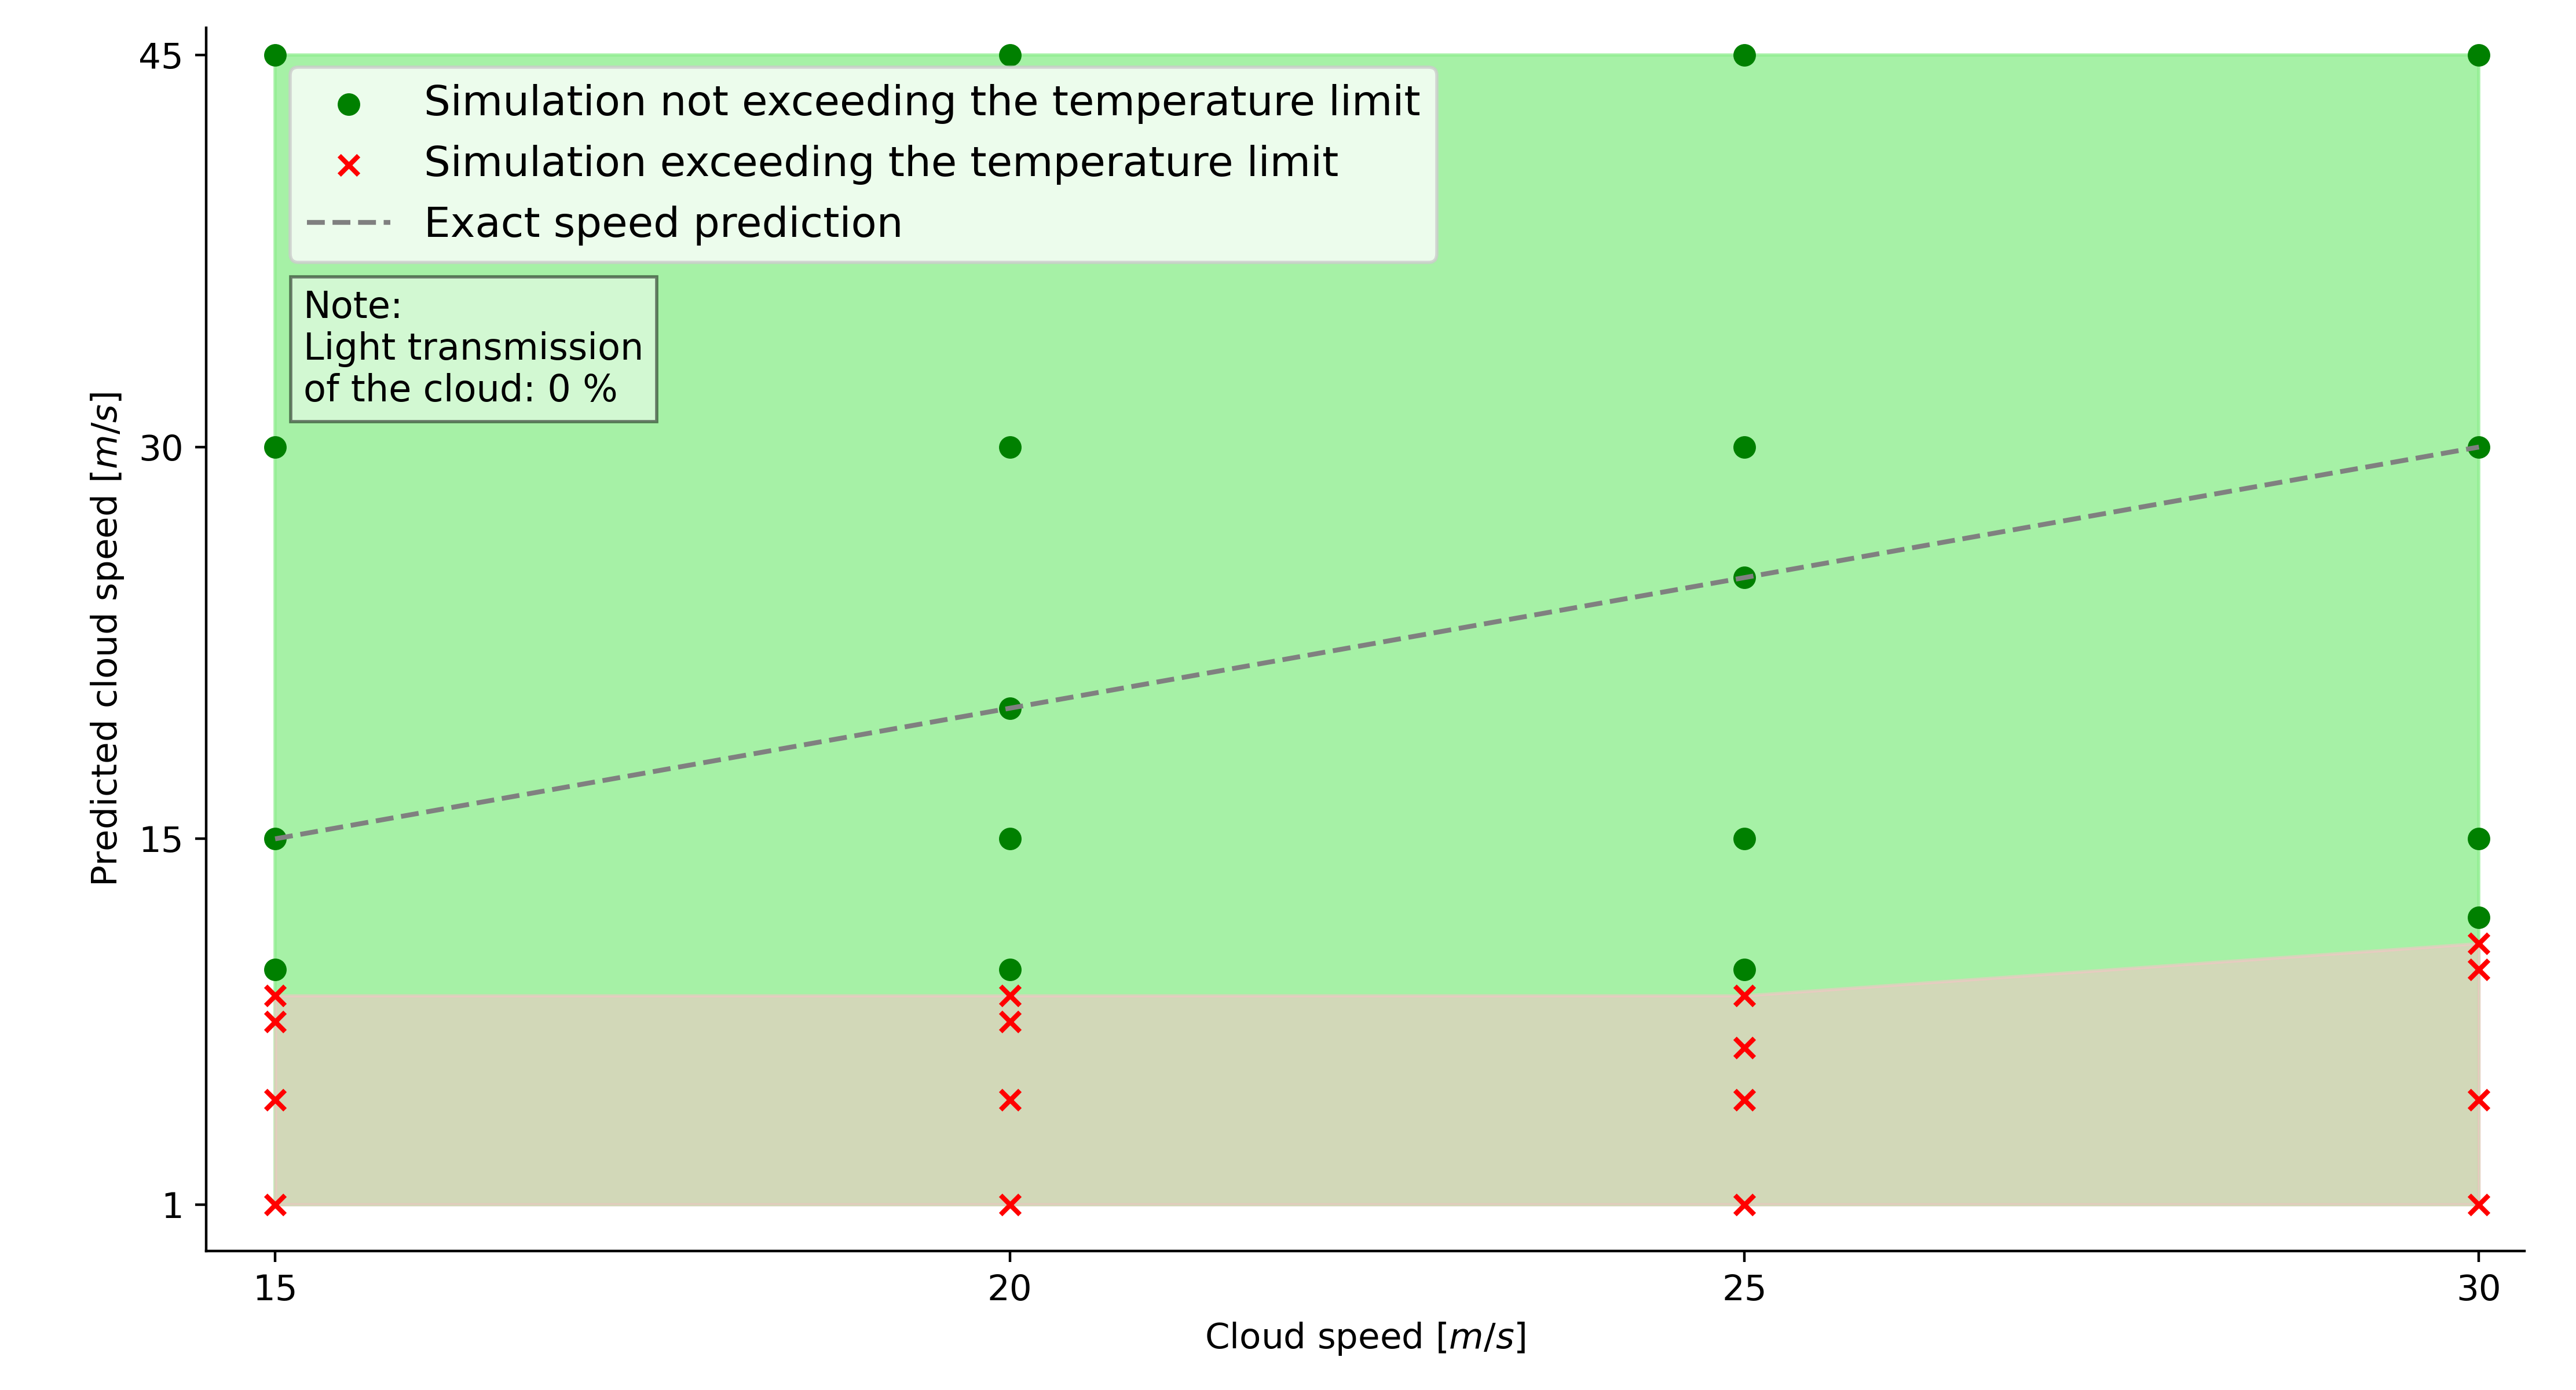
\includegraphics[width=0.99\textwidth]{C:/Users/gesc_ma/VSCode MPC Projekt/dynaovrcontroller/dynaovrcontroller/aimpoint_control_scenarios/plots/21_analyze_speed_uncertainty/safe_simulations_shading_0.png}}
    \caption[Analyse der erlaubten Abweichung in der Prädiktion der Wolkengeschwindigkeit für die Lichtdurchlässigkeit von $\SI{0}{\percent}$]{Analyse der erlaubten Abweichung in der Prädiktion der Wolkengeschwindigkeit für die Lichtdurchlässigkeit von $\SI{0}{\percent}$}
    \label{fig_speed00}
\end{figure}

\begin{figure}[h!]
    \centering
    \setlength{\fboxsep}{1pt}
    \setlength{\fboxrule}{1pt}
    \fbox{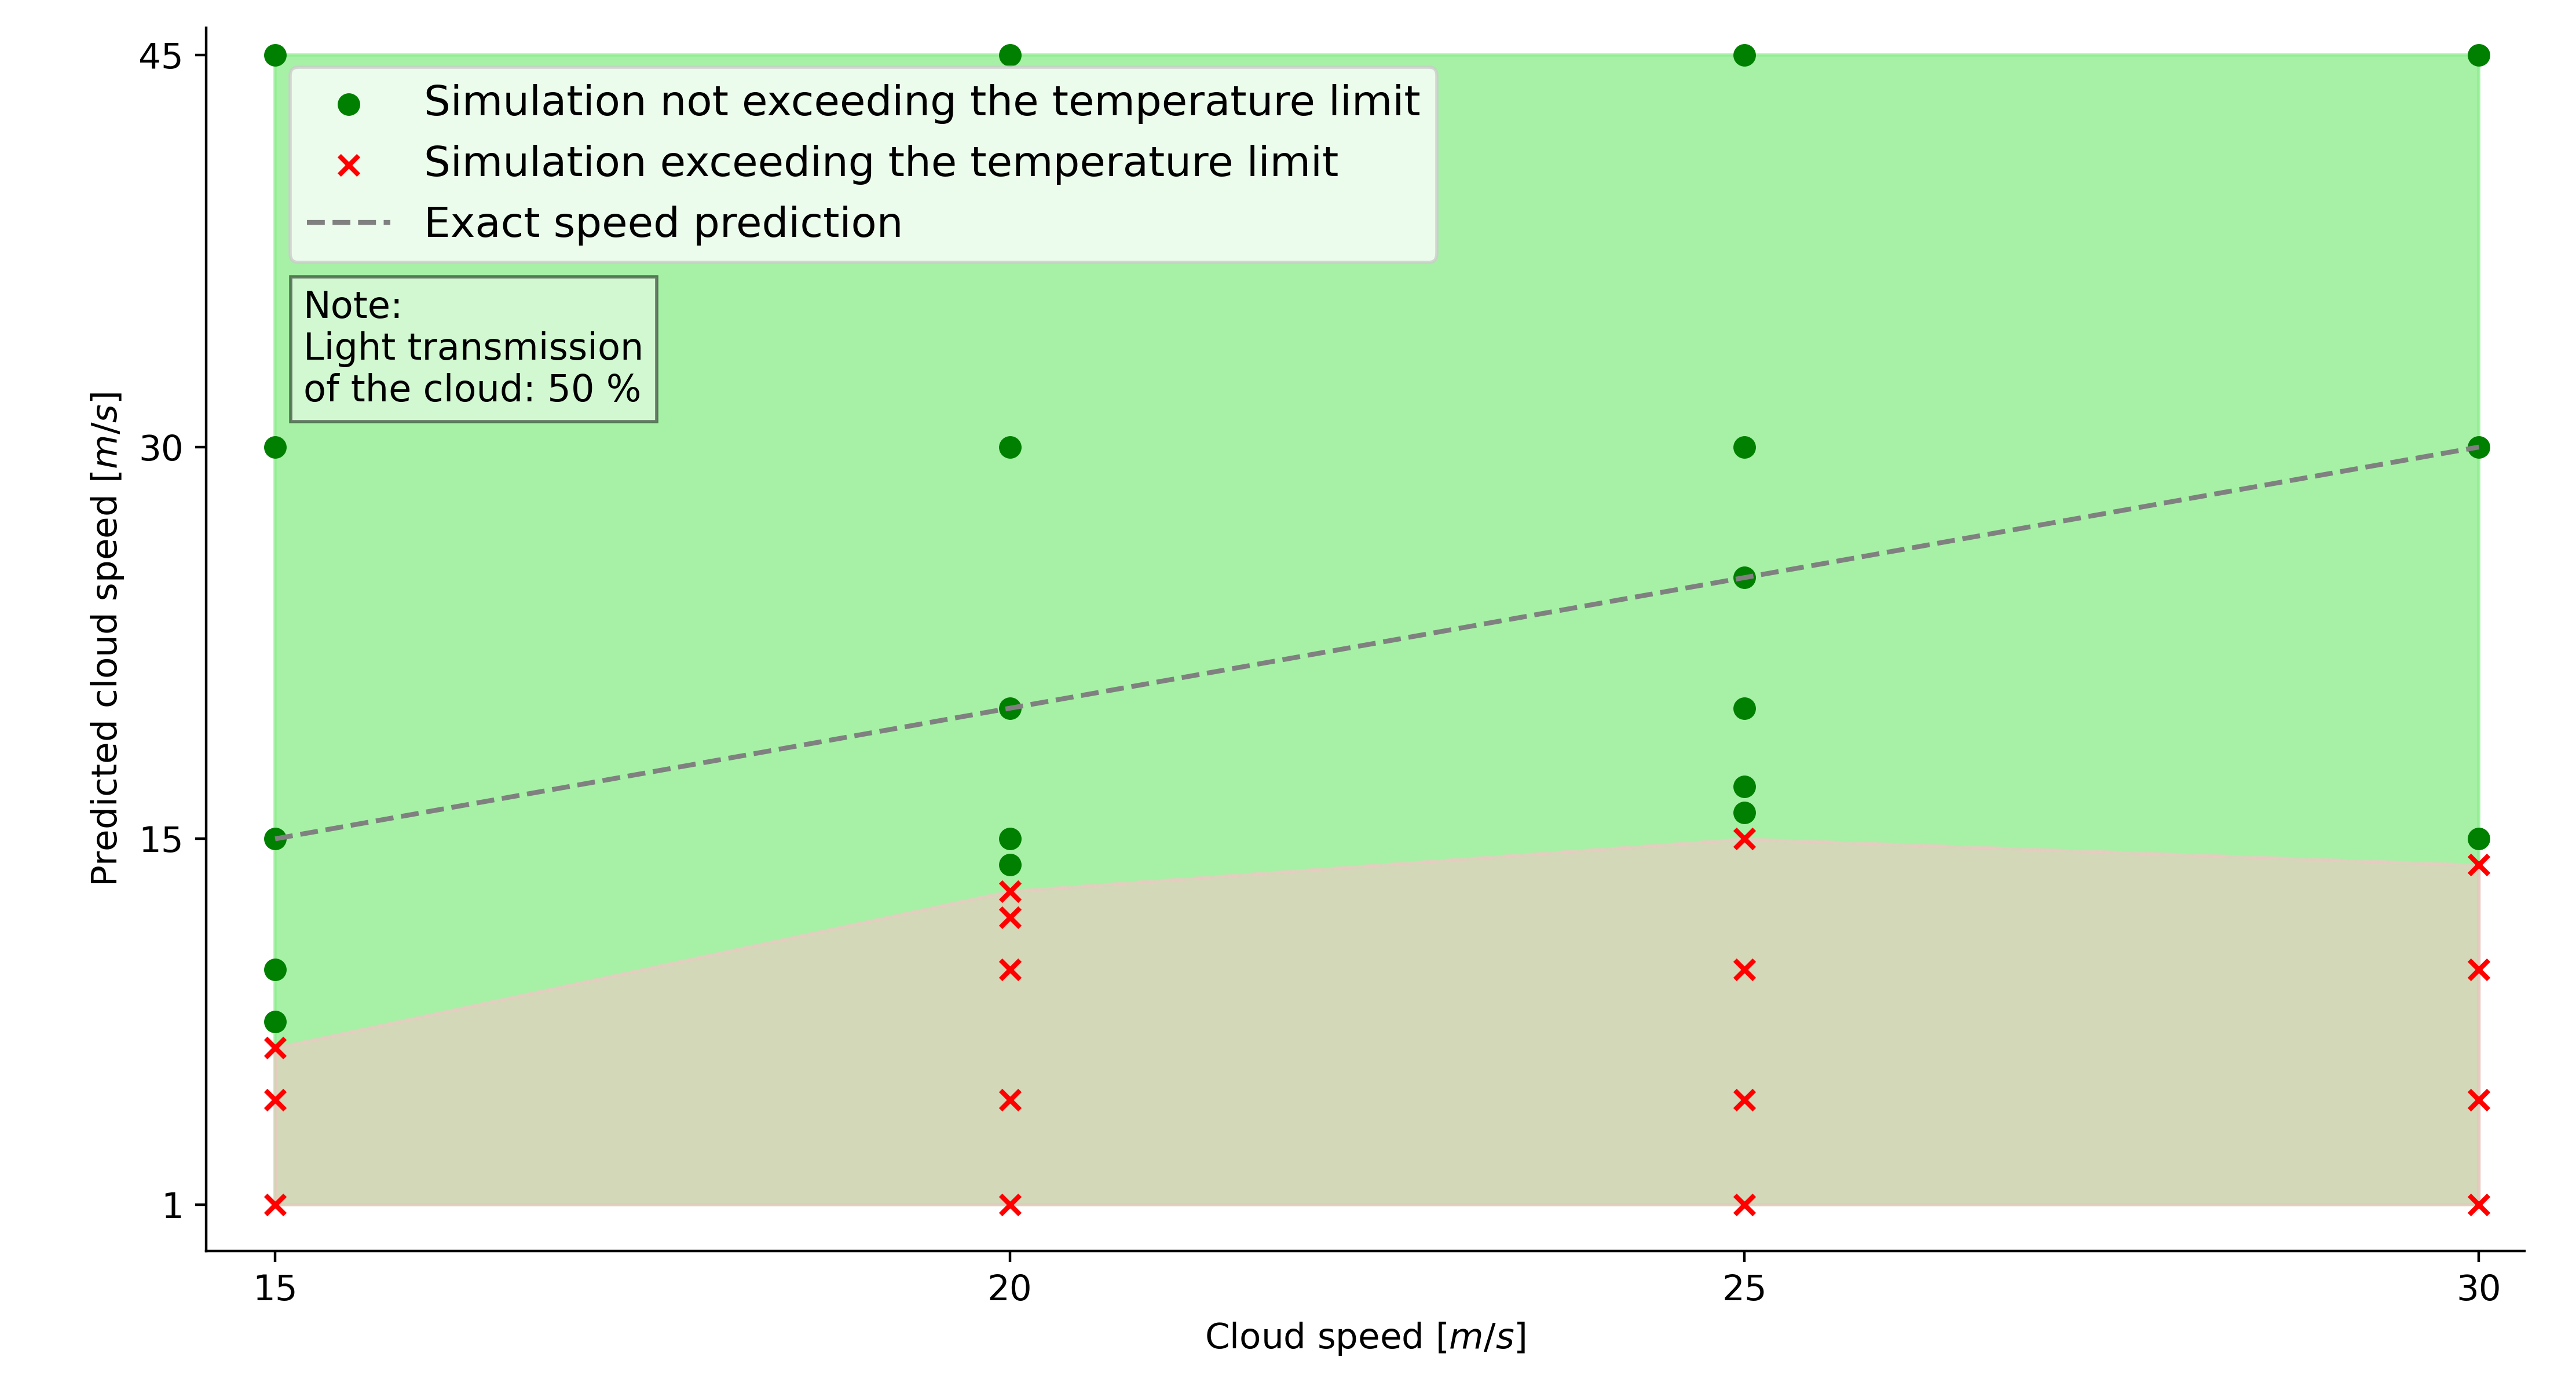
\includegraphics[width=0.99\textwidth]{C:/Users/gesc_ma/VSCode MPC Projekt/dynaovrcontroller/dynaovrcontroller/aimpoint_control_scenarios/plots/21_analyze_speed_uncertainty/safe_simulations_shading_50.png}}
    \caption[Analyse der erlaubten Abweichung in der Prädiktion der Wolkengeschwindigkeit für die Lichtdurchlässigkeit von $\SI{50}{\percent}$]{Analyse der erlaubten Abweichung in der Prädiktion der Wolkengeschwindigkeit für die Lichtdurchlässigkeit von $\SI{50}{\percent}$}
    \label{fig_speed50}
\end{figure}

\begin{figure}[h!]
    \centering
    \setlength{\fboxsep}{1pt}
    \setlength{\fboxrule}{1pt}
    \fbox{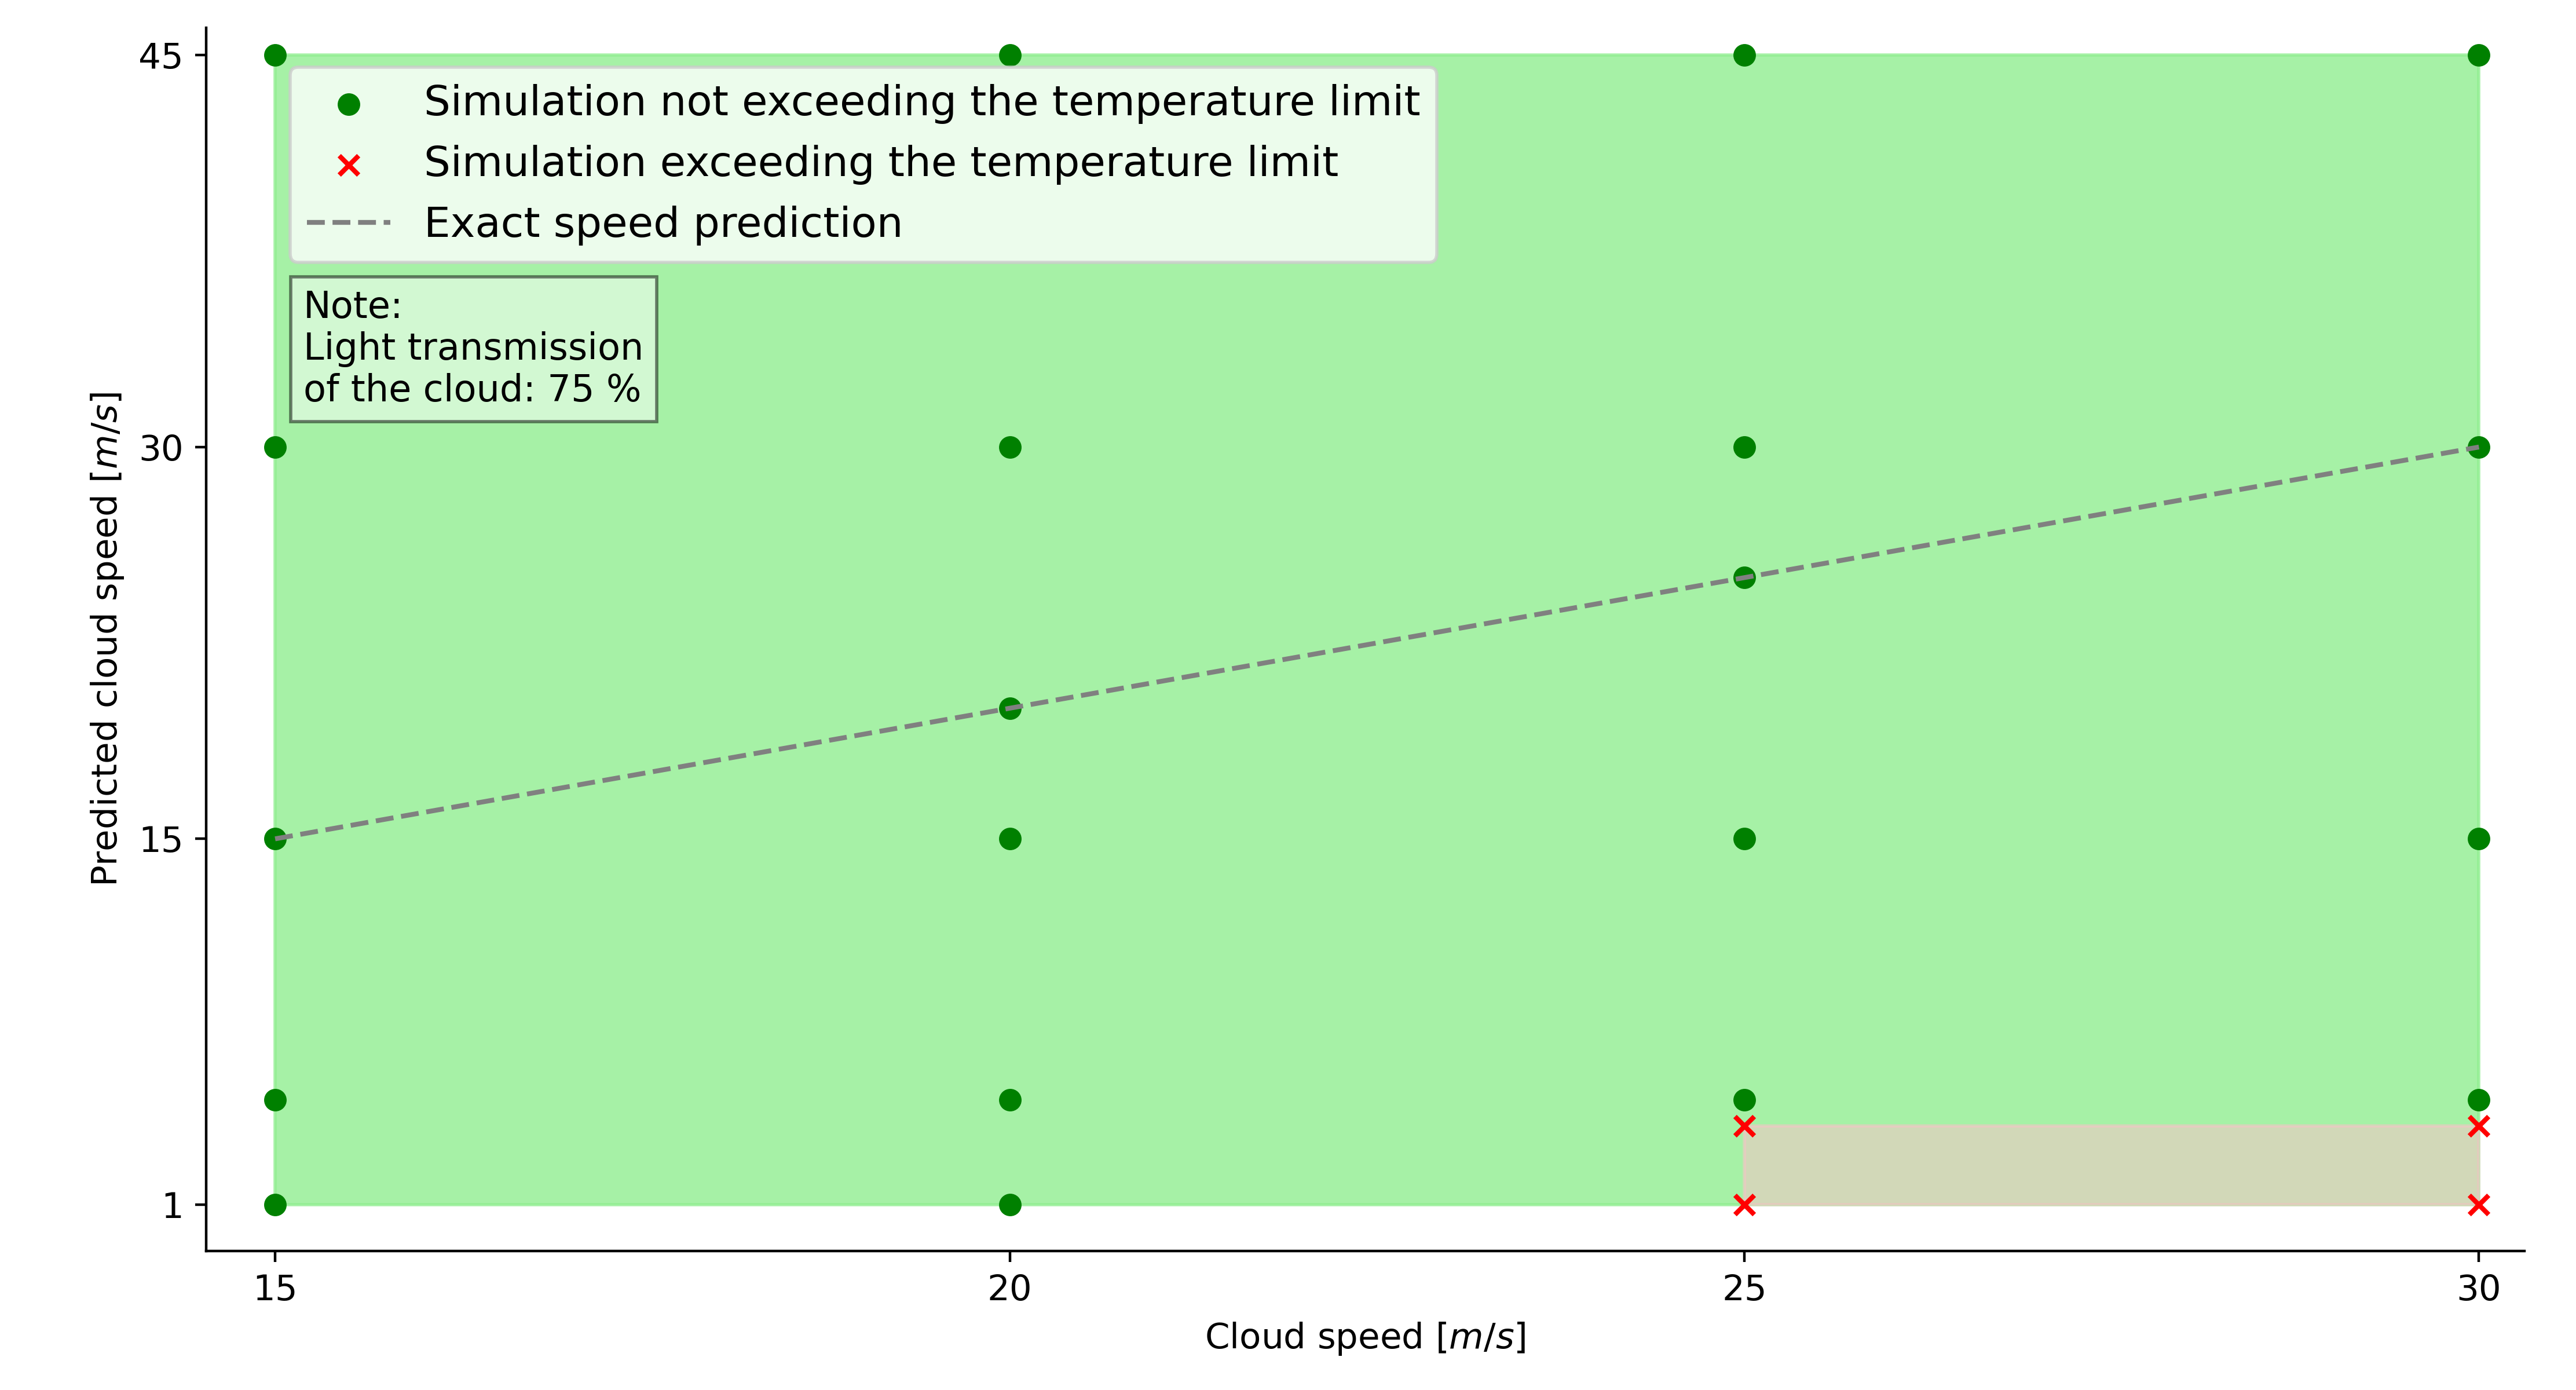
\includegraphics[width=0.99\textwidth]{C:/Users/gesc_ma/VSCode MPC Projekt/dynaovrcontroller/dynaovrcontroller/aimpoint_control_scenarios/plots/21_analyze_speed_uncertainty/safe_simulations_shading_75.png}}
    \caption[Analyse der erlaubten Abweichung in der Prädiktion der Wolkengeschwindigkeit für die Lichtdurchlässigkeit von $\SI{75}{\percent}$]{Analyse der erlaubten Abweichung in der Prädiktion der Wolkengeschwindigkeit für die Lichtdurchlässigkeit von $\SI{75}{\percent}$}
    \label{fig_speed75}
\end{figure}

\begin{figure}[h!]
    \centering
\setlength{\fboxsep}{1pt}
\setlength{\fboxrule}{1pt}
\fbox{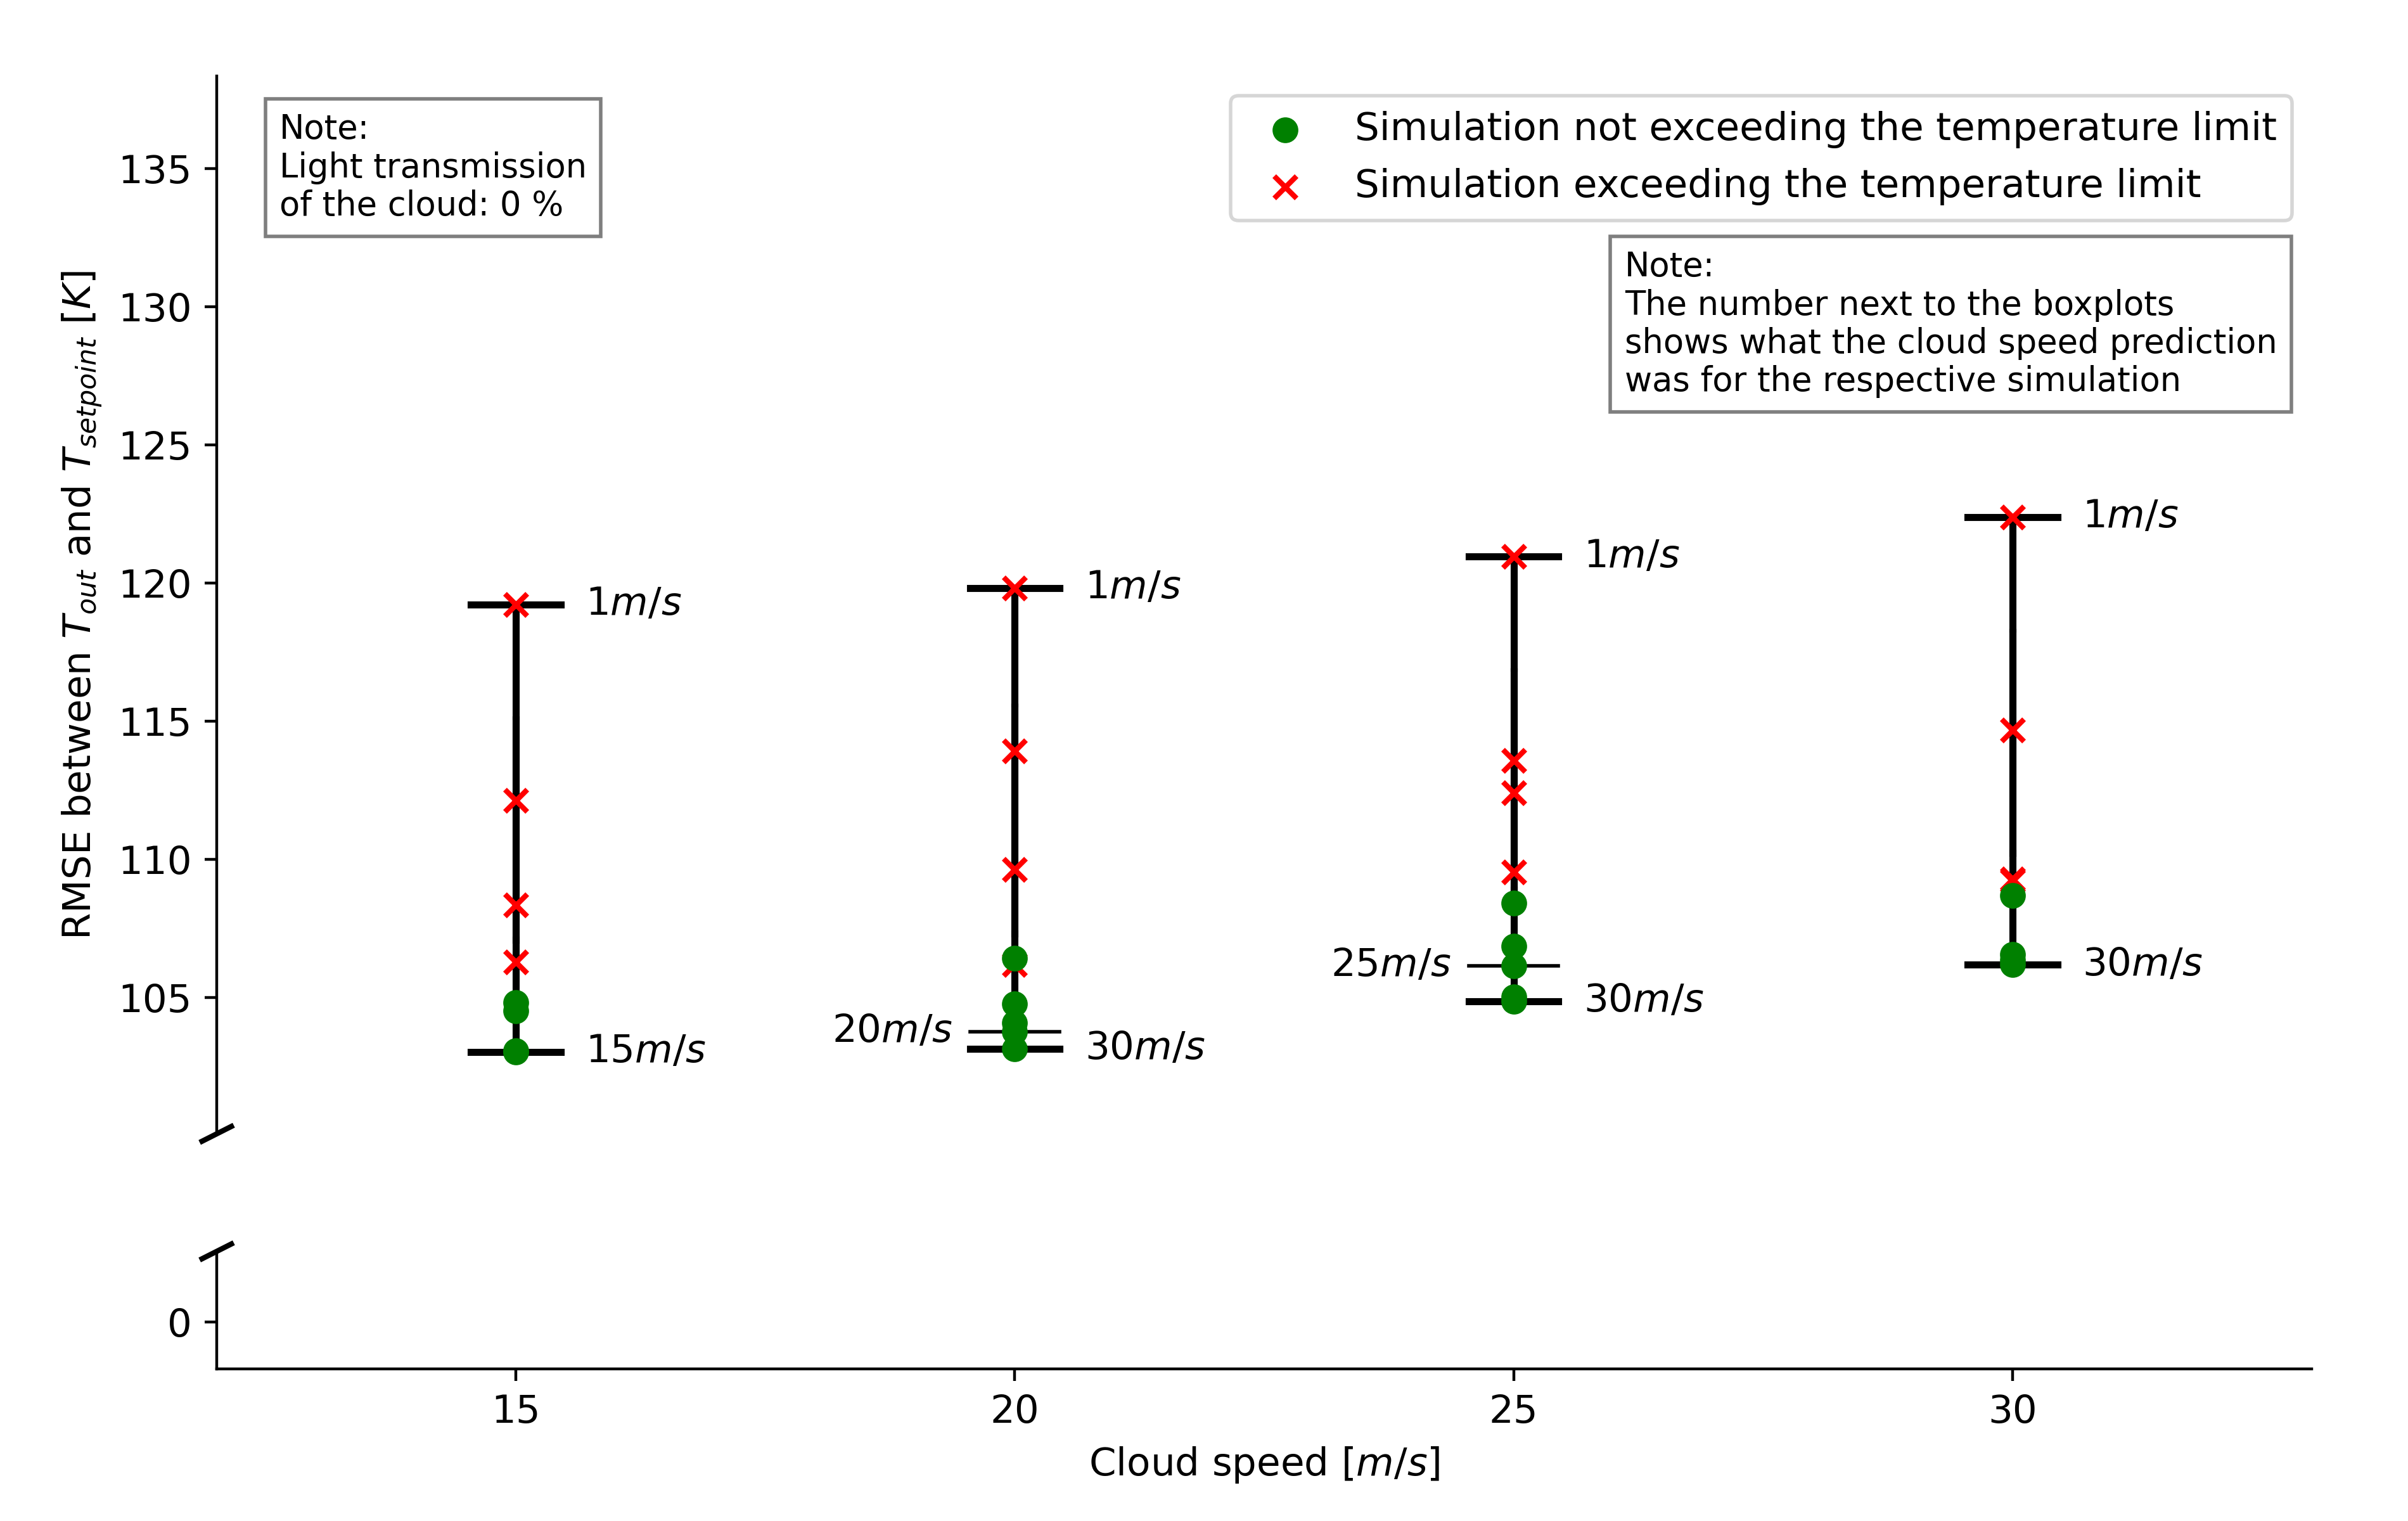
\includegraphics[width=0.99\textwidth]{C:/Users/gesc_ma/VSCode MPC Projekt/dynaovrcontroller/dynaovrcontroller/aimpoint_control_scenarios/plots/21_analyze_speed_uncertainty/rmse_per_speed_shading_0.png}}
\caption[Analyse des RMSE für unterschiedliche Prädiktionen der Wolkengeschwindigkeiten für die Lichtdurchlässigkeit der Wolke von $\SI{0}{\percent}$]{Analyse des RMSE für unterschiedliche Prädiktionen der Wolkengeschwindigkeiten für die Lichtdurchlässigkeit der Wolke von $\SI{0}{\percent}$}
\label{fig_speed00RMSE}
\end{figure}

\begin{figure}[h!]
    \centering
\setlength{\fboxsep}{1pt}
\setlength{\fboxrule}{1pt}
\fbox{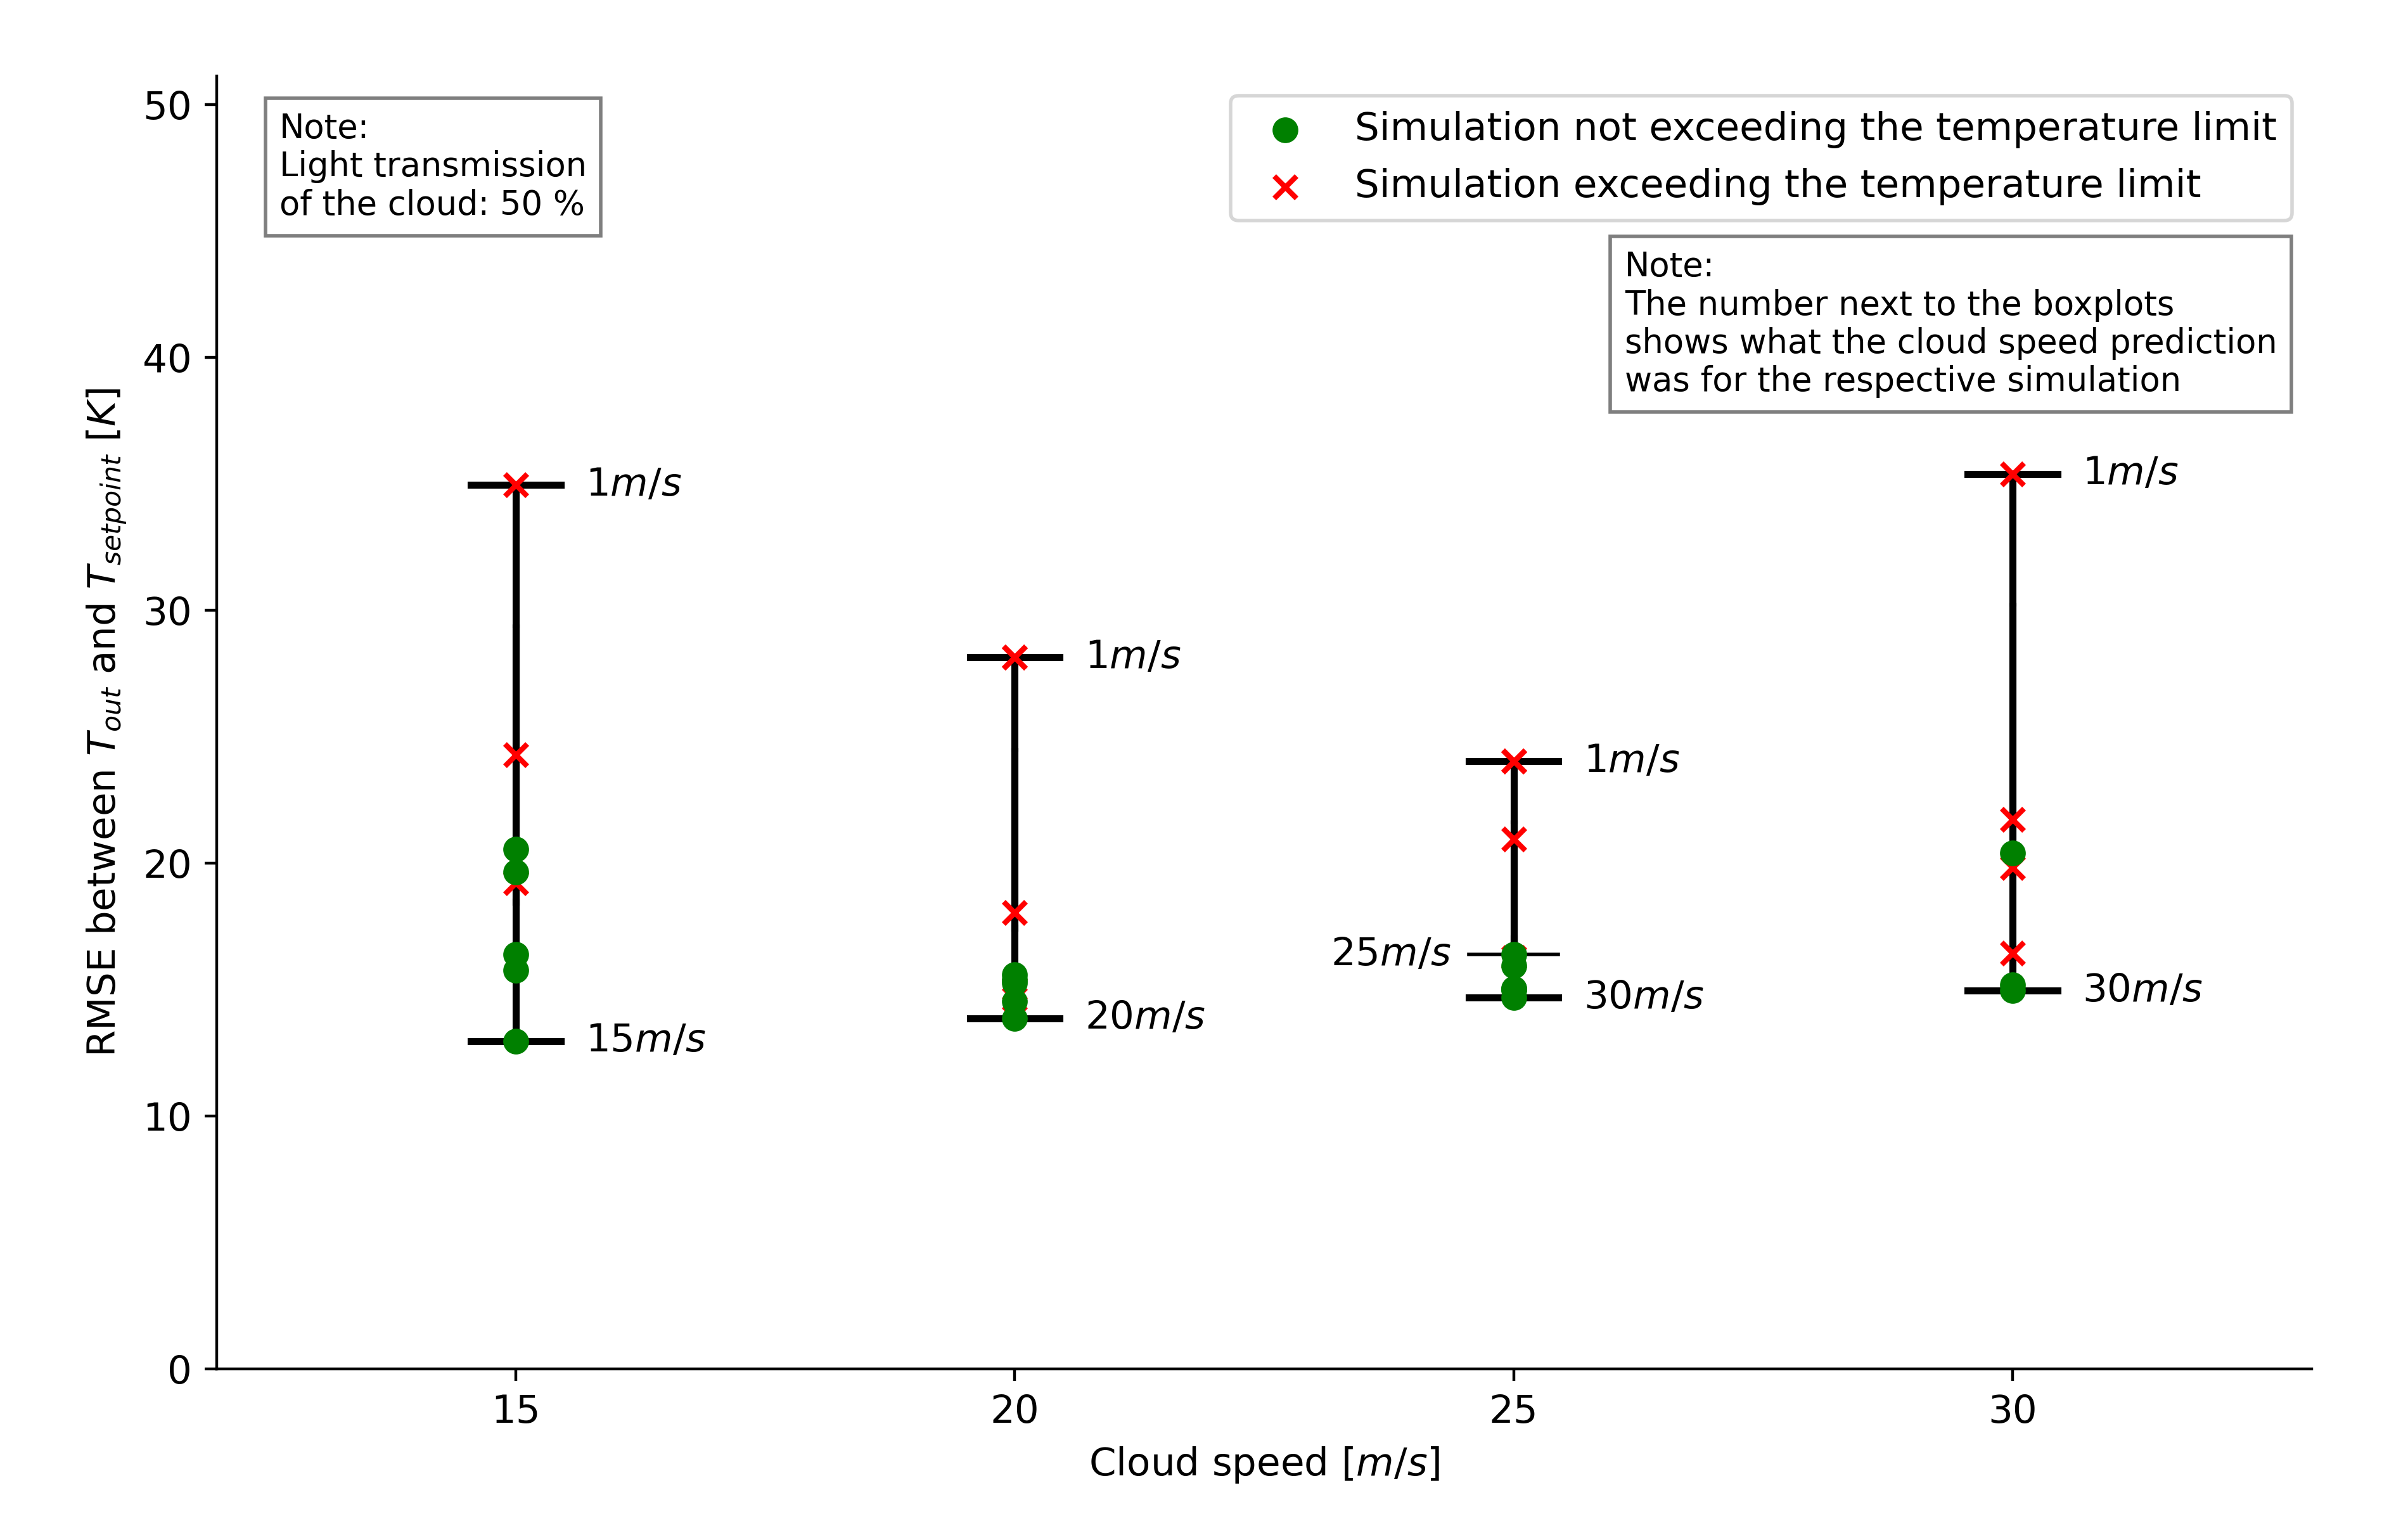
\includegraphics[width=0.89\textwidth]{C:/Users/gesc_ma/VSCode MPC Projekt/dynaovrcontroller/dynaovrcontroller/aimpoint_control_scenarios/plots/21_analyze_speed_uncertainty/rmse_per_speed_shading_50.png}}
\caption[Analyse des RMSE für unterschiedliche Prädiktionen der Wolkengeschwindigkeiten für die Lichtdurchlässigkeit der Wolke von $\SI{50}{\percent}$]{Analyse des RMSE für unterschiedliche Prädiktionen der Wolkengeschwindigkeiten für die Lichtdurchlässigkeit der Wolke von $\SI{50}{\percent}$}
\label{fig_speed50RMSE}
\end{figure}

\begin{figure}[h!]
    \centering
    \setlength{\fboxsep}{1pt}
    \setlength{\fboxrule}{1pt}
    \fbox{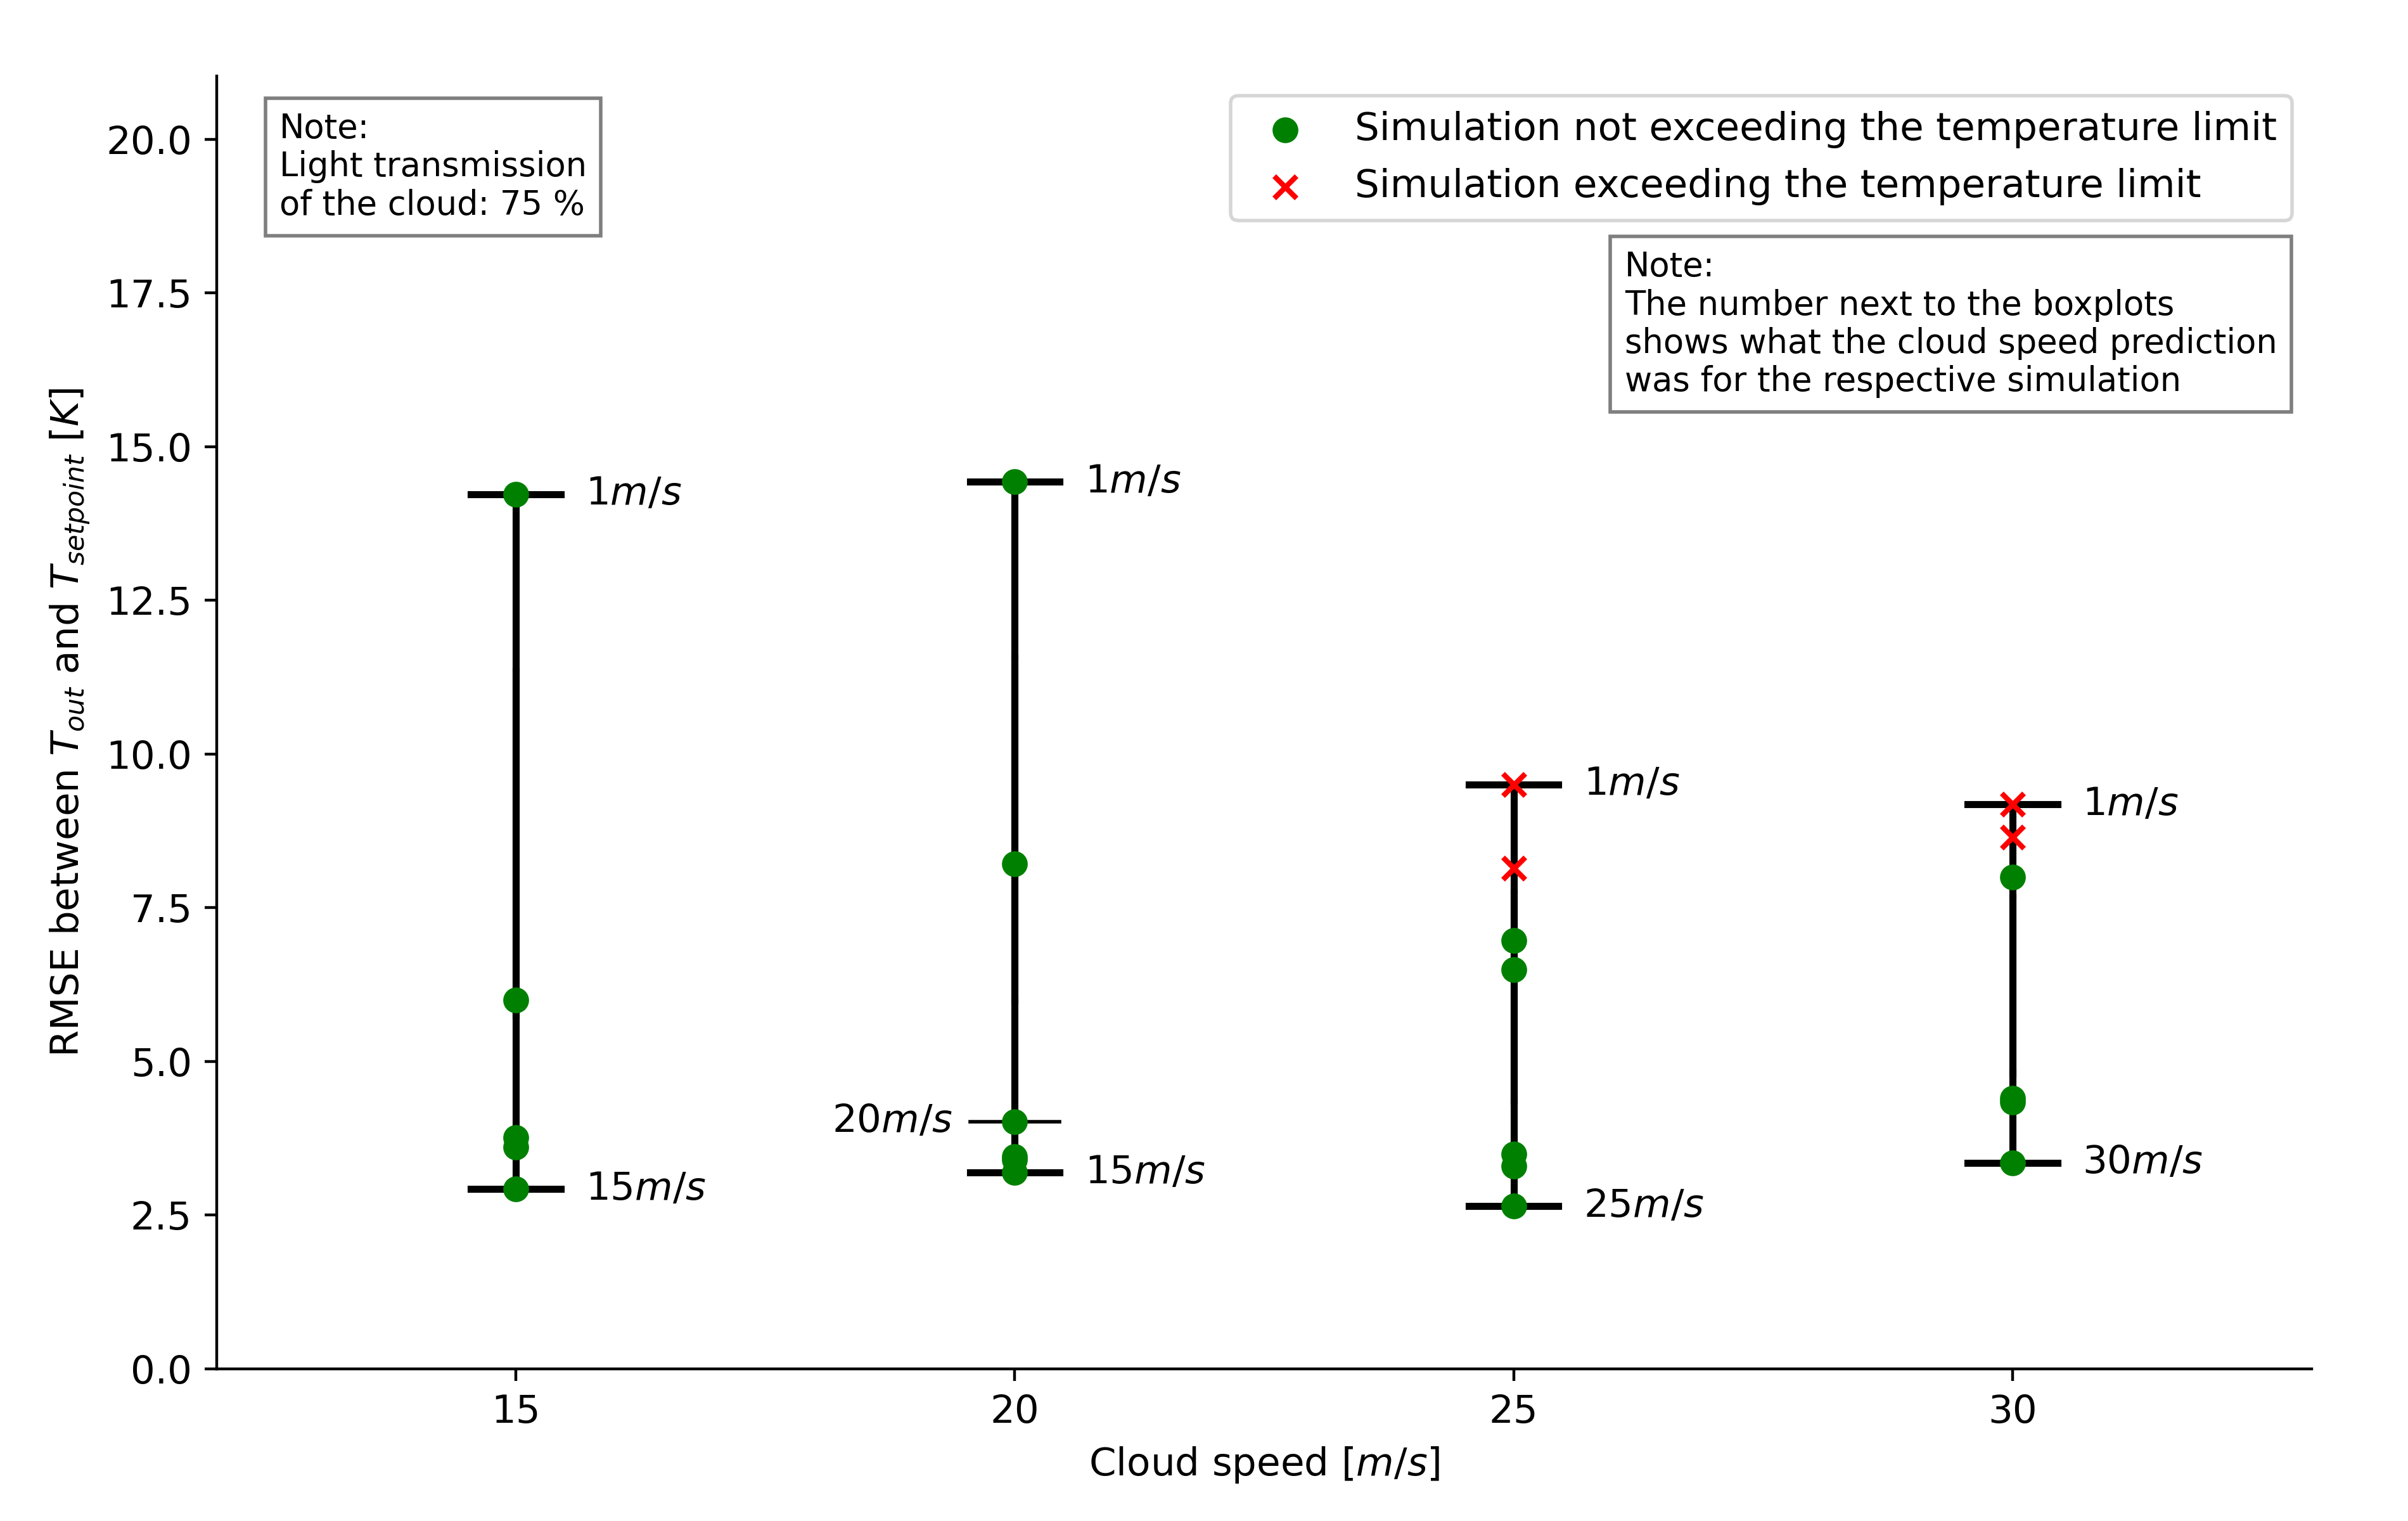
\includegraphics[width=0.89\textwidth]{C:/Users/gesc_ma/VSCode MPC Projekt/dynaovrcontroller/dynaovrcontroller/aimpoint_control_scenarios/plots/21_analyze_speed_uncertainty/rmse_per_speed_shading_75.png}}
    \caption[Analyse des RMSE für unterschiedliche Prädiktionen der Wolkengeschwindigkeiten für die Lichtdurchlässigkeit der Wolke von $\SI{75}{\percent}$]{Analyse des RMSE für unterschiedliche Prädiktionen der Wolkengeschwindigkeiten für die Lichtdurchlässigkeit der Wolke von $\SI{75}{\percent}$}
    \label{fig_speed75RMSE}
\end{figure}

\begin{figure}[t]
    \centering
    \setlength{\fboxsep}{1pt}
    \setlength{\fboxrule}{1pt}
    \fbox{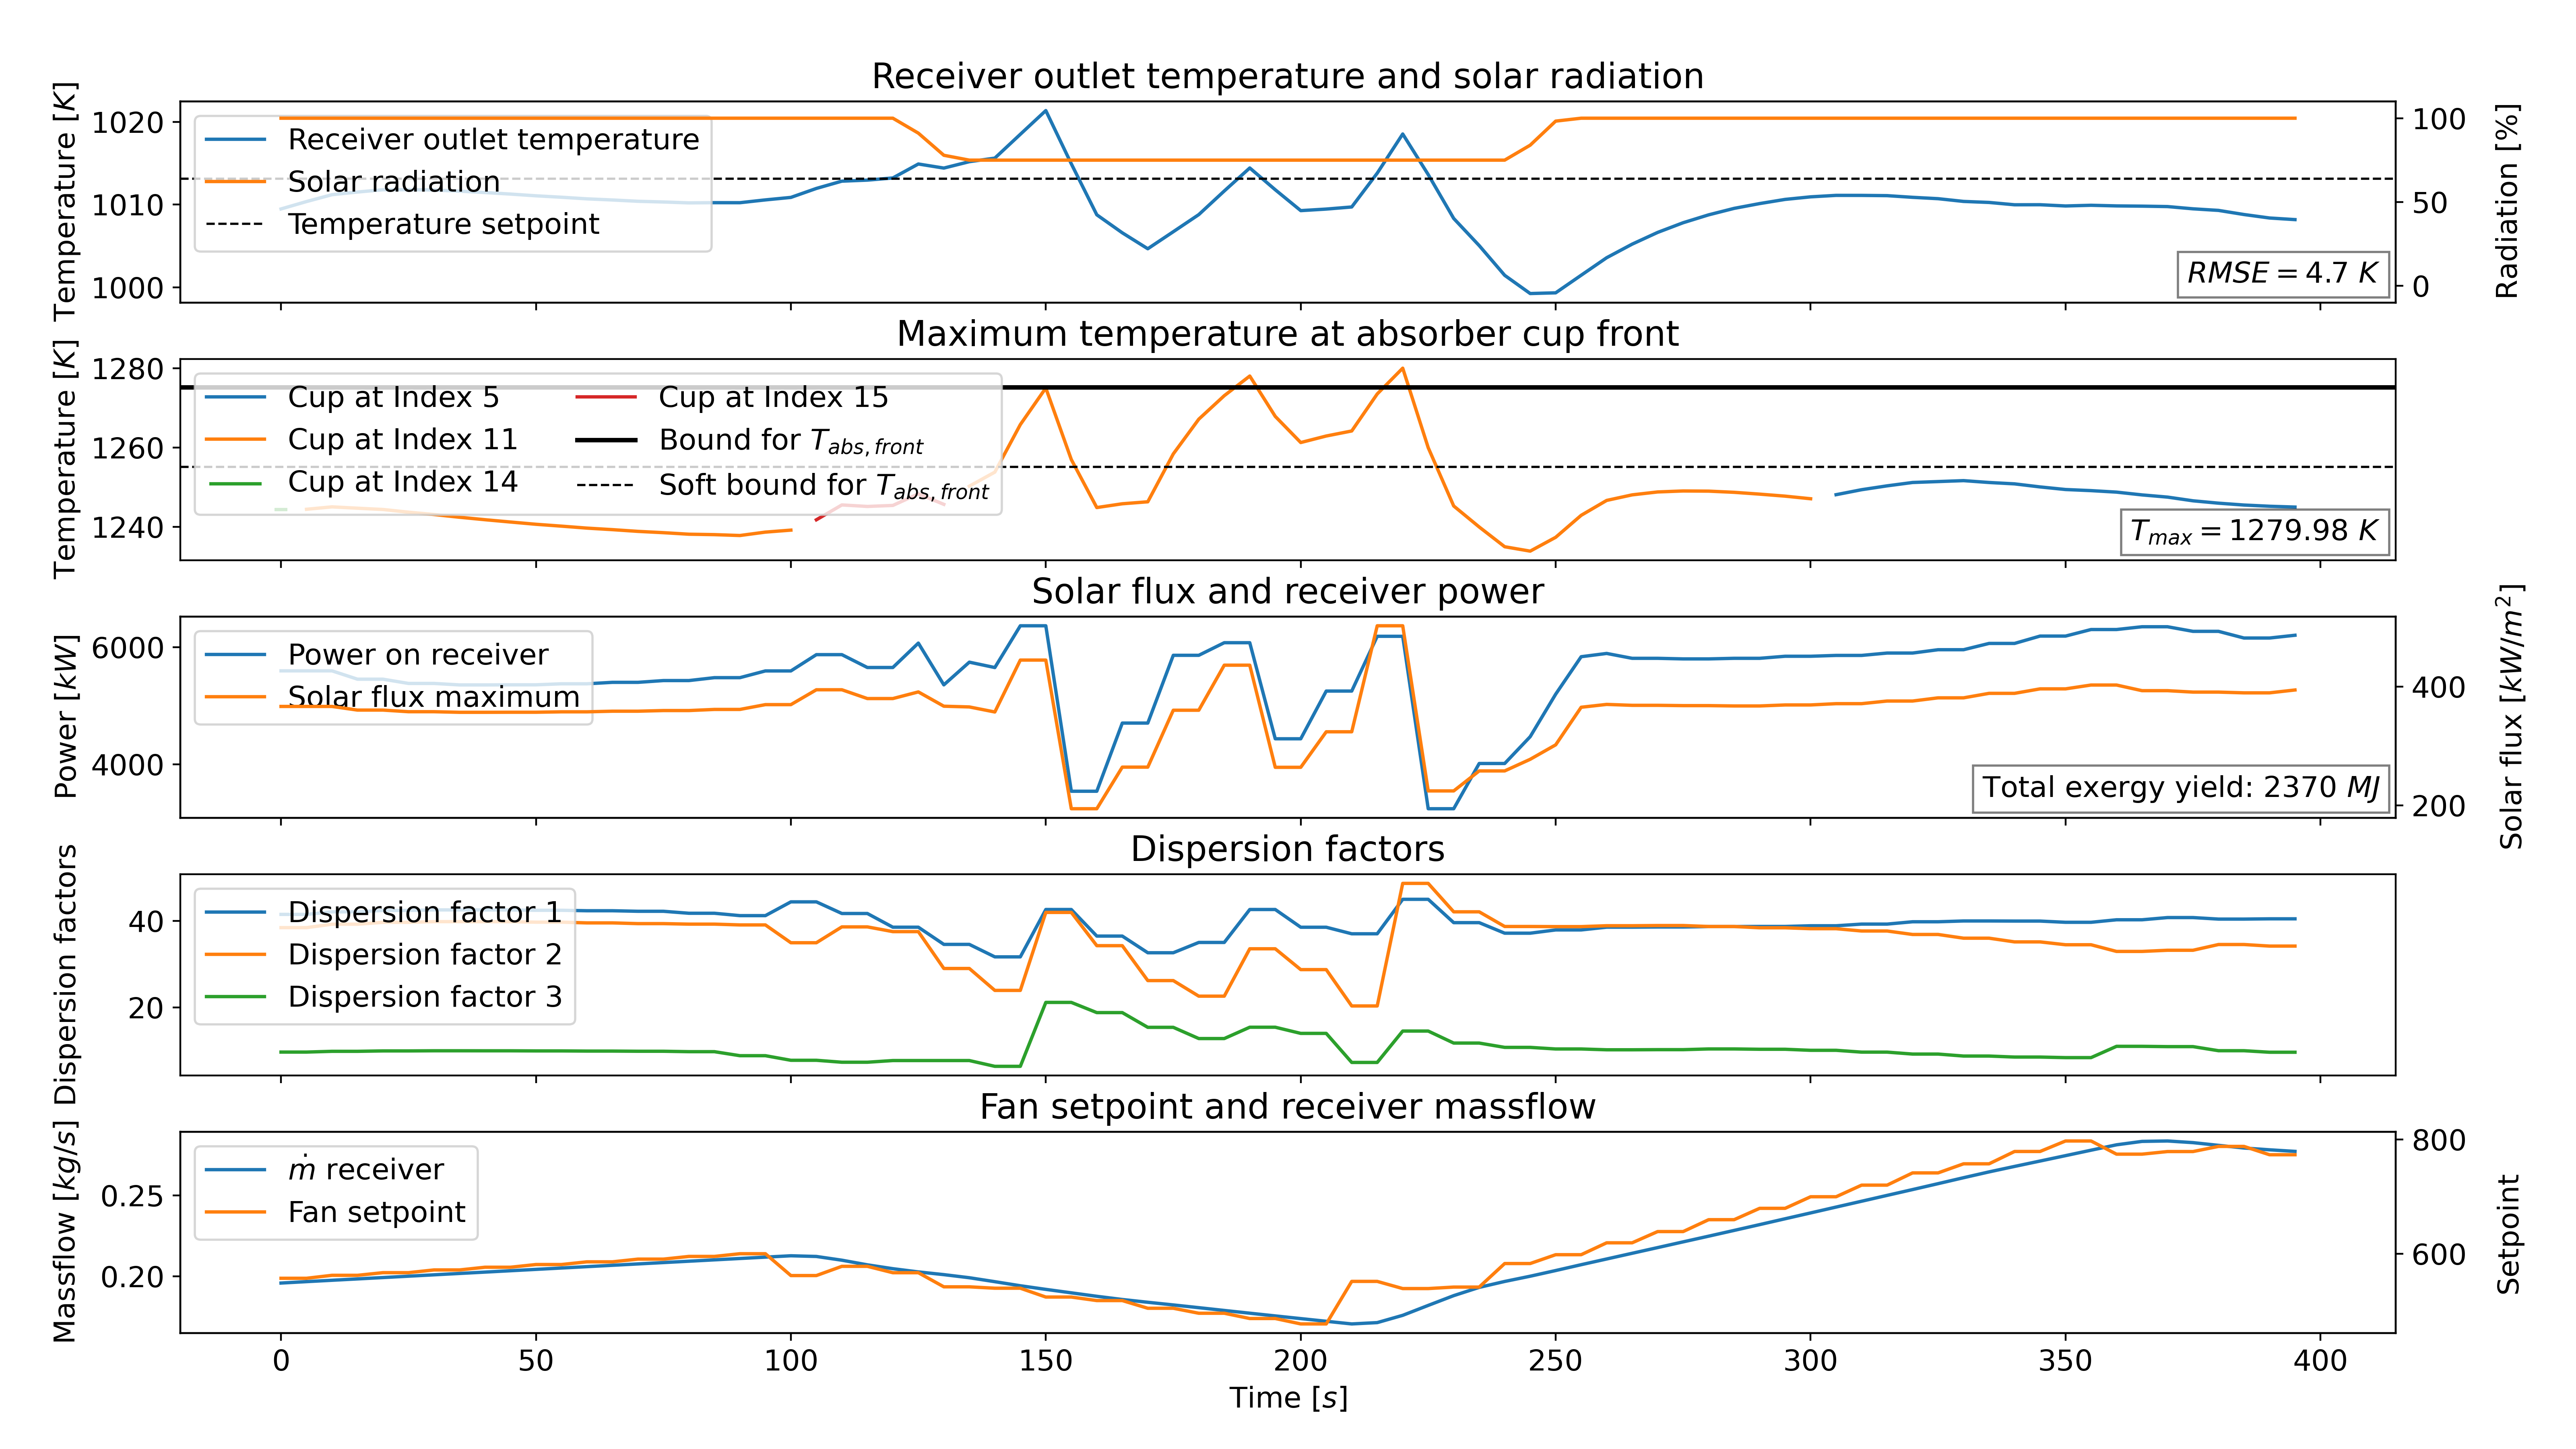
\includegraphics[width=0.99\textwidth]{C:/Users/gesc_ma/VSCode MPC Projekt/dynaovrcontroller/dynaovrcontroller/aimpoint_control_scenarios/plots/04_mpc_uncertain_information_shading/75/shading_120sec_75_30mps_thinking_50.png}}
\caption[Simulationsverlauf mit Wolkengeschwindigkeit $\SI{30}{\metre\per\second}$ und Lichtdurchlässigkeit von $\SI{75}{\percent}$ bei Vorhersage von $\SI{0}{\percent}$]{Simulationsverlauf mit Wolkengeschwindigkeit $\SI{30}{\metre\per\second}$ und Lichtdurchlässigkeit von $\SI{75}{\percent}$ bei Vorhersage von $\SI{0}{\percent}$}
    \label{fig_uncertain753000}
 \end{figure}
